\documentclass{article}
\usepackage[
        a4paper,% other options: a3paper, a5paper, etc
        left=3cm,
        right=3cm,
        top=3cm,
        bottom=4cm,
        % use vmargin=2cm to make vertical margins equal to 2cm.
        % us  hmargin=3cm to make horizontal margins equal to 3cm.
        % use margin=3cm to make all margins  equal to 3cm.
]{geometry}
%\usepackage[utf8x]{inputenc}
\usepackage{graphicx}
\usepackage{caption}
\usepackage{enumerate}
\usepackage{subcaption}
\usepackage[procnames]{listings}
\usepackage{color}
\usepackage{amssymb}
\usepackage{amsmath}
\usepackage{comment}
\usepackage{hyperref}
\usepackage{blindtext}
\usepackage[titletoc,title]{appendix}
\usepackage{float}
\usepackage{fullpage}
\definecolor{codegreen}{rgb}{0,0.6,0}
\definecolor{codegray}{rgb}{0.5,0.5,0.5}
\definecolor{codepurple}{rgb}{0.58,0,0.82}
\definecolor{backcolour}{rgb}{0.95,0.95,0.92}

\lstdefinestyle{mystyle}{
    backgroundcolor=\color{backcolour},
    commentstyle=\color{codegreen},
    keywordstyle=\color{magenta},
    numberstyle=\tiny\color{codegray},
    stringstyle=\color{codepurple},
    basicstyle=\ttfamily,
    breakatwhitespace=false,
    breaklines=true,
    captionpos=t,
    keepspaces=true,
    numbers=left,
    numbersep=5pt,
    showspaces=false,
    showstringspaces=false,
    showtabs=false,
    tabsize=2
}

\lstset{style=mystyle, language=Matlab}

\title{Computer Vision - Lab 1}
\author{Luuk Boulogne (s2366681) \and Steven Bosch (s1861948)}
\date{\today}

\begin{document}
\maketitle

\section{Parameter effects}
The following subsections discuss the parameter influence for both of the vector field methods. We use the initial settings as standard settings and will change one parameter at the time to see its influence on the performance.

For the standard settings (with 200 iterations) we see that the standard vector field method results in a snake that finds the shape except for the cavity, while the gradient vector flow method finds the u-shape very nicely.

\subsection{Smoothing}
When we smooth the image the edges get blurred, which causes the area around the edges to contain values higher than zero. Therefore we the standard external force vector field has non zero vectors in a greater area in the image, further away from the edges themselves. 

We expect that because of this, in the standard vector field method, a smoothed image will make it possible for more snake initializations to approximate the shape. For example, if the snake gets initialized within a shape too far away from the edges, in a non-blurred image the snake misses vectors to extract it due to the lack of external force. For a smoothed image, the range of the influence of the edges has increased and thus snakes can be initialized further away from the edges and still find the approximate shape. The results show us that this is indeed the case, for example for a $\sigma$ of 5, a snake initialized within the 'u' shape, still finds a solution if it at some point touches a force vector.

Another result we found for the standard method when using a smoothed image ($\sigma = 5$ is that the cavity is depicted better. This is probably due to the fact that instead of only horizontal opposite force vectors, these force vectors now get a direction downwards due to the influence of the bottom edge of the cavity.

With the GVF method stronger edge map gradients are retained in the vector force field, while weaker gradients are smoothed out, as predicted in the energy formulation in equation 12 of the paper. Therefore we expect that for higher smoothing values (for which edge map gradients are weaker) the GVF method ignores these to some extent, which causes the snake to non-accurately represent the shape in the image. This is indeed what we can observe when we use a smoothed image for a $\sigma = 5$.

\subsection{Regularization parameter GVF and iteration parameter}
The regularization parameter $\mu$ and the iteration parameter cause the influence of the edge force vectors to be `stretched' out over a wider area, so that in areas further away from an edge there also appear force vectors in the direction of that edge. So in a non-smoothed image, for a wide range of initializations of the snake to work, we need to set $\mu$ and the iteration parameter high enough so that (preferably) the whole image has force vectors in the right direction. However, if we set the parameters too high, the influence of the edge force vectors will interfere with each other, causing the snake to not work properly.

When we test the parameter this is largely the effect we see. If we use $\mu = 0.1$ and $iterations = 100$, the snake finds the u-shape very nicely (also for higher radius snakes), since the influence of the edge force vectors is well distributed over the image. However, if we use $\mu = 0$, a snake of radius 0.5 does not find the cavity and a snake of radius 0.8 takes very long, since initially it only has the internal force pulling it in the right direction, since there are no force vectors in the area around the shape. On the other hand if we use $\mu = 1$ the snake does not find the shape either, due to the interference effect we mentioned above.

\subsection{Alpha}
Alpha controls the part of the internal force of the snake that represents tension. Therefore, when alpha is large, we expect two things. Firstly, the snake contracts with a stronger force and therefore the circomference becomes smaller more easily. Secondly, irregularities in the edge of the shape are ignored. For very large values of alpha, even the cavity of the u shape might be ignored.

When we test the parameter, we indeed find these effects. The larger alpha is, the more time it takes for the snake to find the cavity and the cavity becomes approximated more poorly.

\subsection{Beta}
Beta controls the part of the internal force of the snake that represents rigidity. Therefore, when beta is large, we expect that more external force is needed to bend the snake and that sharp corners in the snake do therefore not occur. Since there are no sharp edges, we expect beta to have little effect on the eventual shape of the snake, as long as it does not become so large that the rigidity causes the cavity to be ignored.

For GVF, when we test the parameter, we do find the effects mentioned above. When the beta becomes larger, it takes more iterations to approximate the cavity, because more force is needed to bend the snake. At a certain beta, the lowest point in the cavity cannot be reached anymore. After this, the higher beta becomes, the more shallow the cavity is approximated by the snake. This is because it takes more force to bend the snake and therefore the point at which the external force and the internal force becomes equal is at a shape of the snake where the cavity is more shallowly represented. 

For the standard vector force field, the same effects apply, only the cavity is never well approximated in the first place. 

\subsection{Kappa}
Kappa denotes the strenght of the external force field. This means that for small values of kappa, the external force field (the edges in the image) has a small inpact on the snake and for large values, it has a large impact. We therefore expect that for smaller values of kappa the movement of the snake is driven more by its internal forces. This implies that when the snake deforms, the edges in the image are ignored more. For large kappa we expect that due to the large influence of the edges, the snake moves quickly towards the image contours.

When testing the effects of kappa, we found for small kappa our expectations were met. For example, a snake initialized in a circle with radius 0.5 for a kappa of 0.01, the snake just shrinks to a smaller circle. 
We also found that for large kappa, instead of quickly finding the solution, the snake overshoots the edge on every step. This causes it to not converge to the contours. 

\subsection{Resolution of the snake}
Dmin is the minimal resolution of the snake and dmax is the maximal resolution of the snake. These parameters together thus determine the range of possible distances between two adjacent nodes of the snake.

We expect that for the standard vector force field, a range of only large possible distances between two adjacent nodes can cause negative effects: In this case, due to the lack of force vectors at non-edge locations, there are no external forces on nodes that lie in between nodes that are already on edges. An example of this is when there are two nodes on the vertical edges of the fingers and one node in between them. Because of the large distance between the nodes, there are no external forces where the middle node is located. Therefore it remains at its location, while it would be better if it would move towards an edge. 

With GVF, the cavity is found because there are points inbetween the fingers that are pushed down by the external force field. When dmax becomes large enough to allow having two adjacent nodes where one node is on the left finger and one node is on the right finger, there are no nodes inbetween the fingers. Therefore the cavity cannot be found.

Finally, when dmax is small, the snake finds a good solution, but because there are more nodes on the snake, the number of calculations per iteration increases.

When testing the effects of the resolution parameters, the application indeed ran slower with very high resolution snakes. Also the cavity was not found for low resolution GVF snakes as expected. However, we did not find an instance of the first problem mentioned for low resolution snakes using a standard vector force field. This might have to do with the fact that the application does not support initial values of dmin that are higher than 1.

\renewcommand{\thesubsection}{\large{Exercise \arabic{subsection}}}
\section{Exercise questions}
\subsection{}
The most inportant differences in behaviour between GVF and classical snakes for the u shape are the following. 

Firstly, when not smoothing the image, the classical snake cannot approximate the contour of the cavity while the GVF snake can. The classical snake experiences only horizontal forces at the inner edges of the fingers. Therefore it is not propegated into the cavity (see \ref{fig1a}). With GVF, the nodes inbetween the fingers do experience downwards forces and there does succeed in finding the cavity (see \ref{fig1b}).

\begin{figure}[H]
\centering
\begin{subfigure}{0.49\textwidth}
  \centering
  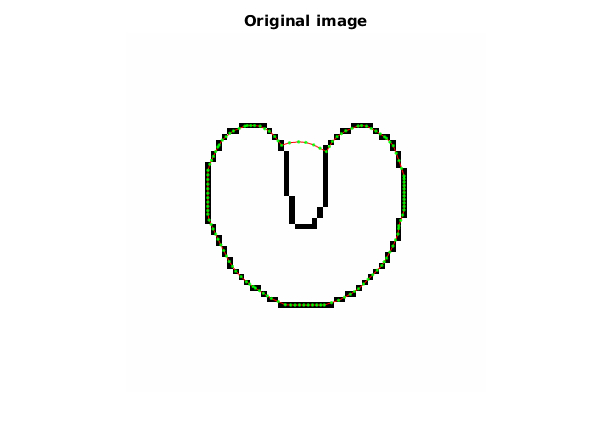
\includegraphics[width=\linewidth]{fig1.png}
  \caption{The U-shape using the classical snake ($\alpha=0.05, \beta=0, \gamma=1,\kappa=0.6,Dmin=0.5,Dmax=2,Iterat=400$).}
  \label{fig1a}
\end{subfigure}
\begin{subfigure}{0.49\textwidth}
  \centering
  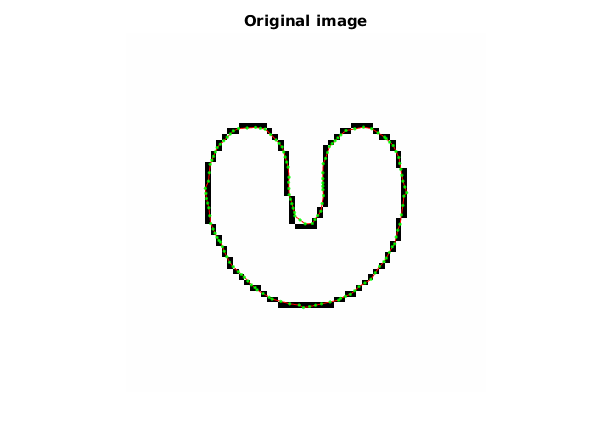
\includegraphics[width=\linewidth]{fig2.png}
  \caption{The U-shape using the GVF snake ($\mu=0.1, Iterations=90, \alpha=0.05, \beta=0, \gamma=1,\kappa=0.6,Dmin=0.5,Dmax=2,Iterat=400$).}
  \label{fig1b}
\end{subfigure}
\caption{Results for the non-smoothed image of the U-shape.}
\end{figure}

Furthermore if the snake is initialized within the U-shape, the GVF can sometimes still find the right solution, because there is an external force field within the shape. The classical snake however, if initialized too far from the edges, can never find the right shape, because of the lack of force vectors. Instead it shrinks down because of the internal force. See also figure \ref{fig2}.

\begin{figure}[H]
\centering
\begin{subfigure}{0.49\textwidth}
  \centering
  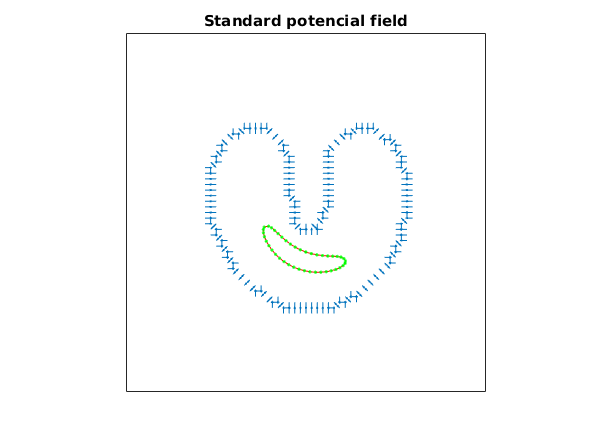
\includegraphics[width=\linewidth]{fig2a.png}
  \caption{Initializing the classical snake within the U-shape places it outside of any external force field.}
  \label{fig2a}
\end{subfigure}
\begin{subfigure}{0.49\textwidth}
  \centering
  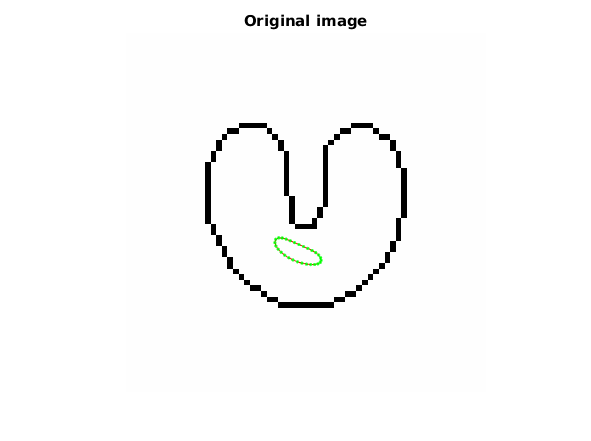
\includegraphics[width=\linewidth]{fig2b.png}
  \caption{Results of the classical snake when initialized within the U-shape after 400 iterations ($\alpha=0.05, \beta=0, \gamma=1,\kappa=0.6,Dmin=0.5,Dmax=2,Iterat=400$).}
  \label{fig2b}
\end{subfigure}
\begin{subfigure}{0.49\linewidth}
  \centering
  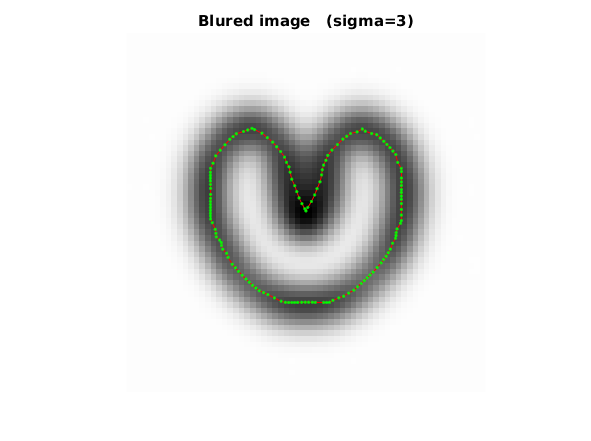
\includegraphics[width=\linewidth]{fig3.png}
  \caption{Results of the classical snake for a smoothed image with $\sigma=3$ ($\alpha=0.05, \beta=0, \gamma=1,\kappa=0.6,Dmin=0.5,Dmax=2,Iterat=400$).}
  \label{fig2c}
\end{subfigure}
\caption{Initializing the snake within the U-shape.}
\label{fig2}
\end{figure}

Also, because of the small capture range of the classical snake with respect to the GVF snake, the classical snake converges more slowly than the GVF snake when it is initialized as a large circle around the u shape. 

We consider the GVF snake to perform better than the classical snake because of the reasons mentioned above. 

Finally, as stated above, the classical snake does not converge into the 'dip' unless image is smoothed with a large enough sigma (see figure \ref{fig2c}). GVF is also able to converge into the 'dip' when the image is not smoothed (figure \ref{fig1b}).



\subsection{}
If the snakes are initialized as a circle around the room, classical snakes converge very well, given enough iterations. GVF snakes need less iterations to converge, but they represent the corners in the figure less accurately. This is because of the smoothing term in equation 12 of the paper. This smoothing causes the force vectors around a corner to point towards the location where the force vectors pointing towards the perpendicular edges are averaged.

\begin{figure}[H]
\centering
\begin{subfigure}{0.49\textwidth}
  \centering
  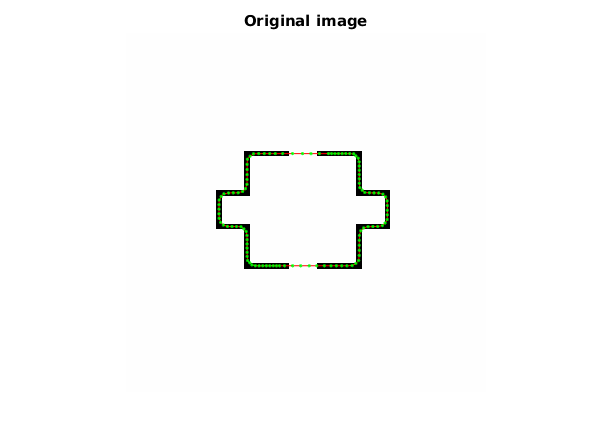
\includegraphics[width=\linewidth]{fig3a.png}
  \caption{The room-shape using the classical snake ($\alpha=0.05, \beta=0, \gamma=1,\kappa=0.6,Dmin=0.5,Dmax=2,Iterat=1000$).}
  \label{fig3a}
\end{subfigure}
\begin{subfigure}{0.49\textwidth}
  \centering
  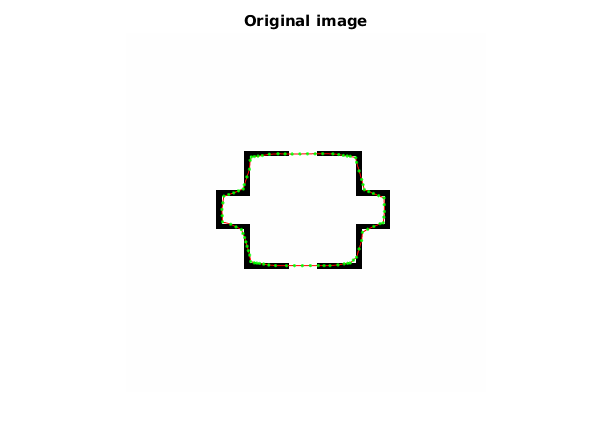
\includegraphics[width=\linewidth]{fig3b.png}
  \caption{The room-shape using the GVF snake ($\mu=0.1, Iterations=90, \alpha=0.05, \beta=0, \gamma=1,\kappa=0.6,Dmin=0.5,Dmax=2,Iterat=400$).}
  \label{fig3b}
\end{subfigure}
\begin{subfigure}{0.49\textwidth}
  \centering
  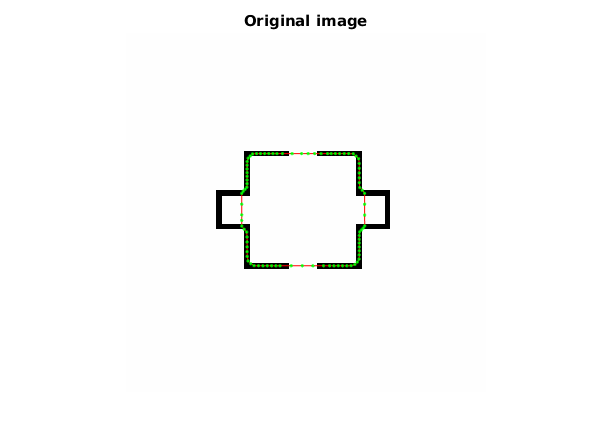
\includegraphics[width=\linewidth]{fig3c.png}
  \caption{The room-shape using a classical snake with a smaller radius than the room ($\mu=0.1, Iterations=90, \alpha=0.05, \beta=0, \gamma=1,\kappa=0.6,Dmin=0.5,Dmax=2,Iterat=1000$).}
  \label{fig3c}
\end{subfigure}
\caption{Results for the non-smoothed image of the room-shape.}
\label{fig3}
\end{figure}

The performance of the GVF is quite robust with respect to the initialization, while the classical snake is not. If (a part of) the left and/or right niche is not inside the initialized snake, the classical snake does not approximate the shape of the niche correctly. This is because of the same reason as that it was unable to find the cavity in the u shape as explained in exercise 1.

\subsection{}
When using the classical snake, the shape of the lungs is not approximated well for any parameter setting, without smoothing the image first. When the image is smoothed with $\sigma$ = 3, the left edge of the left lung and almost the entire right lung are approximated well (see figure \ref{fig4}). This is because the smoothing causes the radius in which an edge causes force vectors to point towards it to become larger. Even though the entire snake is initialized within the lung and therefore the internal forces do not automatically cause the snake to converge towards the shape, when the image is smoothed external forces are enough in this case to propagate the nodes of snake towards the edges.

\begin{figure}[H]
\centering
\begin{subfigure}{0.49\textwidth}
  \centering
  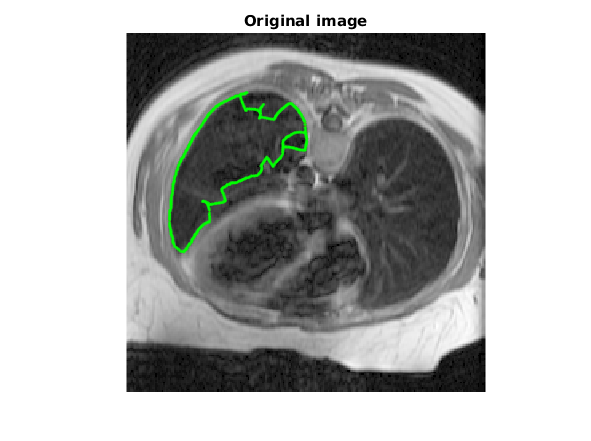
\includegraphics[width=\linewidth]{chestLeftclassical.png}
  \caption{The left chest at convergence ($\alpha=0.05, \beta=0, \gamma=1,\kappa=0.6,Dmin=0.5,Dmax=2,Iterat=400$).}
  \label{fig4a}
\end{subfigure}
\begin{subfigure}{0.49\textwidth}
  \centering
  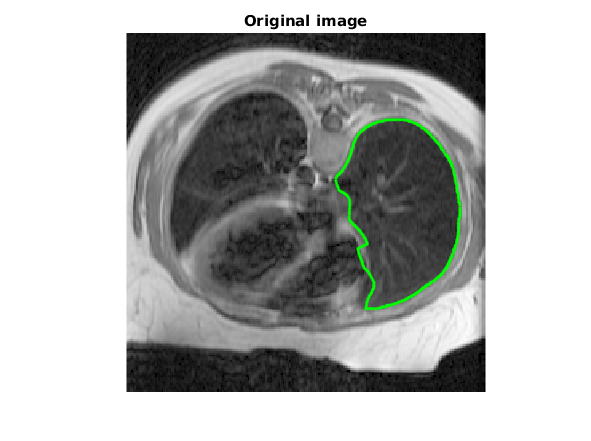
\includegraphics[width=\linewidth]{chestRightclassical.png}
  \caption{The right chest at convergence ($\alpha=0.05, \beta=0, \gamma=1,\kappa=0.6,Dmin=0.5,Dmax=2$).}
  \label{fig4b}
\end{subfigure}
\begin{subfigure}{0.49\textwidth}
  \centering
  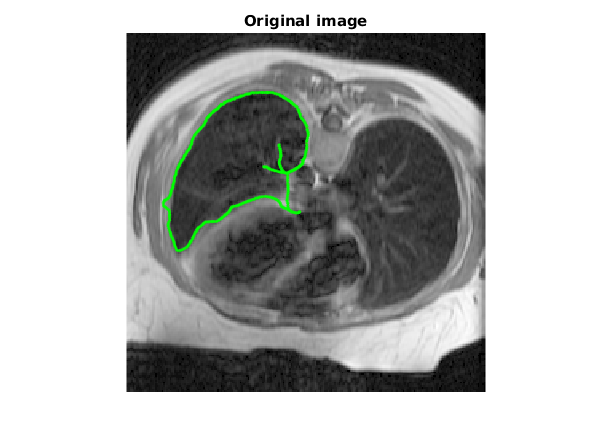
\includegraphics[width=\linewidth]{chestLeftGFV.png}
  \caption{The left chest at convergence ($\mu=0.1, Iterations=90, \alpha=0.05, \beta=0, \gamma=1,\kappa=0.6,Dmin=0.5,Dmax=2$).}
  \label{fig4c}
\end{subfigure}
\begin{subfigure}{0.49\textwidth}
  \centering
  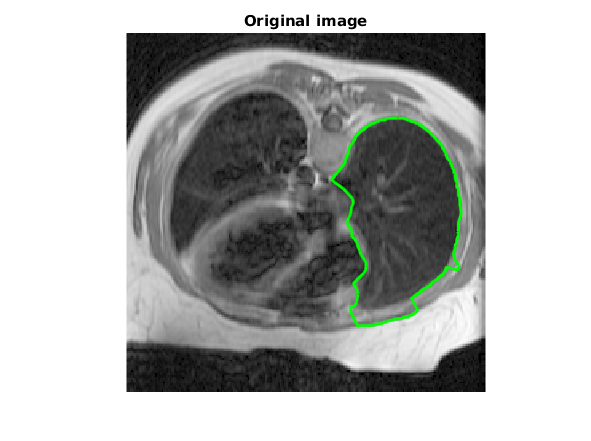
\includegraphics[width=\linewidth]{chestRightGFV.png}
  \caption{The right chest at convergence ($\mu=0.1, Iterations=90, \alpha=0.05, \beta=0, \gamma=1,\kappa=0.6,Dmin=0.5,Dmax=2$).}
  \label{fig4d}
\end{subfigure}
\caption{Results for the smoothed image ($\sigma=3$) of the chest using the classical snake and the non-smoothed image using the GVF snake, using the initial locations of the provided .mat files.}
\label{fig4}
\end{figure}

With GVF, the shape of both lungs can be approximated quite well, even without smoothing (see figure \ref{fig4c} and \ref{fig4d}. This is because now, external forces cause the snake to converge to the shape of the lungs, because of the first term of equation 12 in the paper. There are some edges within the left lung that some nodes of the snake stick to, especially when no smoothing is applied. In the right lung, the bottom edge of the lung is ignored. This is because of the large force caused by the sharper edge below this bottom edge.

\subsection{}
Again, the classical snake did not find a good solution without smoothing, but with smoothing the results were acceptable (see figures \ref{b} and \ref{e}). For the right lung, the right side of the shape is approximated better in the high contrast image, with respect to the original image. This is probably due to the sharper edge. On the left side of the right lung, the shape of the lung is approximated more poorly in the high contrast image. This is due to the detail edges inside the lung that the nodes in the snake stick to.

With GVF again the non-smoothed images provided better results than the smoothed ones (see figures \ref{c} and \ref{f}). For the left lung, the performance was similar. For the right lung, the performance was better in the bottom part, since for the most part, the actual shape of the lung was found instead of the edge below it. However, there are also some new locations on the shape of the lung in which now an edge outside of the lung is found instead of the edge of the lung itself, where this was not the case with the original image.

In both figure \ref{fig4} and \ref{figurebla} we can see loose ends in some locations. To solve this the parameter $\beta$ can be set to a non zero value (e.g. 0.2), which does not alter the overall shape detection, but does remove the lines going inward with a dead end.

\begin{figure}[H]
\centering
\begin{subfigure}{0.45\textwidth}
  \centering
  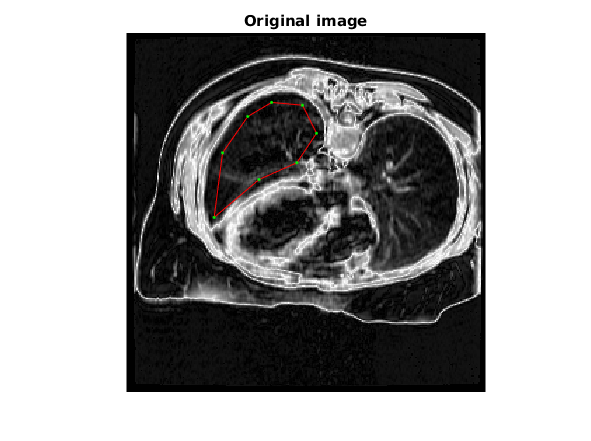
\includegraphics[width=\linewidth]{newLeftinit.png}
  \caption{Left initialization.}
  \label{a}
\end{subfigure}
\begin{subfigure}{0.45\textwidth}
  \centering
  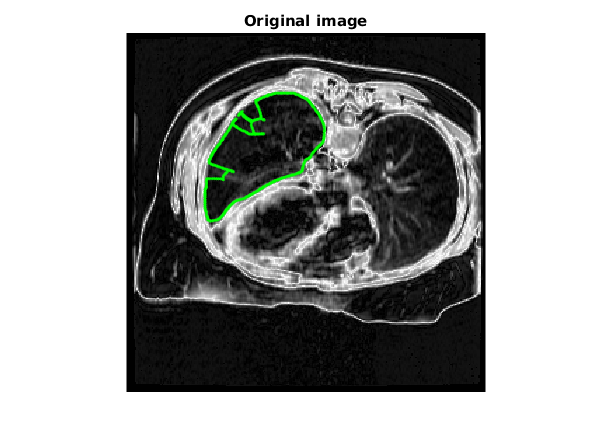
\includegraphics[width=\linewidth]{newLeftclassical.png}
  \caption{Using the classical snake for the right chest at convergence ($\alpha=0.05, \beta=0, \gamma=1,\kappa=0.6,Dmin=0.5,Dmax=2$).}
  \label{b}
\end{subfigure}
\begin{subfigure}{0.45\textwidth}
  \centering
  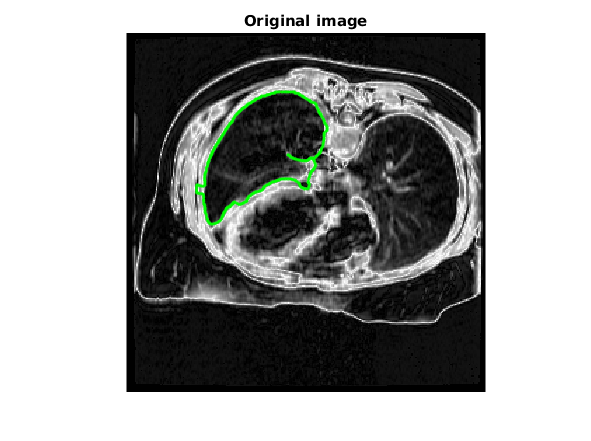
\includegraphics[width=\linewidth]{newLeftGFV.png}
  \caption{Using the GVF snake for the left chest at convergence ($\mu=0.1, Iterations=90, \alpha=0.05, \beta=0, \gamma=1,\kappa=0.6,Dmin=0.5,Dmax=2$).}
  \label{c}
\end{subfigure}
\begin{subfigure}{0.45\textwidth}
  \centering
  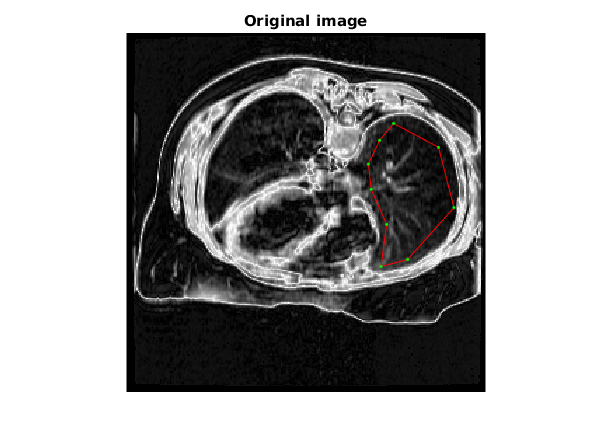
\includegraphics[width=\linewidth]{newRightinit.png}
  \caption{Right initialization.}
  \label{d}
\end{subfigure}
\begin{subfigure}{0.45\textwidth}
  \centering
  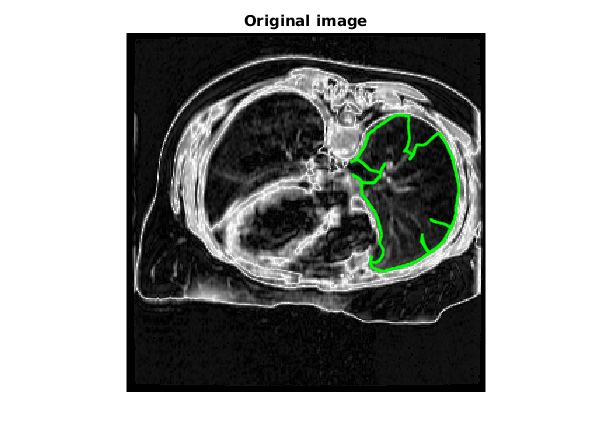
\includegraphics[width=\linewidth]{newRightclassical.png}
  \caption{Using the classical snake for the right chest at convergence ($\alpha=0.05, \beta=0, \gamma=1,\kappa=0.6,Dmin=0.5,Dmax=2$).}
  \label{e}
\end{subfigure}
\begin{subfigure}{0.45\textwidth}
  \centering
  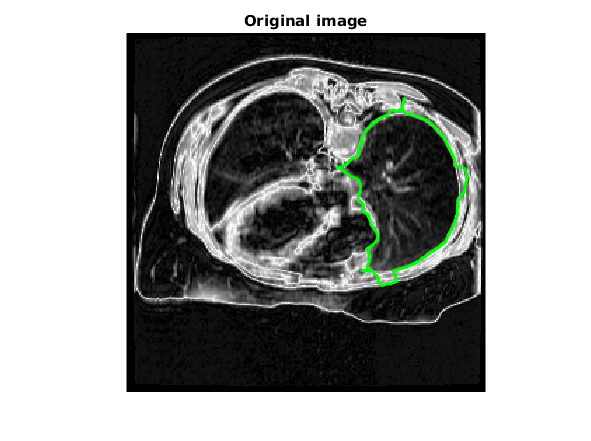
\includegraphics[width=\linewidth]{newRightGFV.png}
  \caption{Using the GVF snake for the right chest at convergence ($\mu=0.1, Iterations=90, \alpha=0.05, \beta=0, \gamma=1,\kappa=0.6,Dmin=0.5,Dmax=2$).}
  \label{f}
\end{subfigure}
\caption{Results for the new image.}
\label{figurebla}
\end{figure}

\subsection{}
Figure \ref{fig6} shows the results for the non-smoothed heart images, using the initializations defined in heart.mat and heart1.mat. The figure shows that the classical snake does not perform very well. This can be well explained by its force vector field, which is shown in figure \ref{fig7a}. As we can observe, the force vectors are `all over the place'. There is no clear direction to be discovered in the force vectors, which is probably caused by the noise in the image. Therefore the resulting snakes (figures \ref{fig6a} and \ref{fig6b}) show no clear smoothed lines.
On the other hand the force vector field of the GVF method shows much clearer patterns (see figure \ref{fig7b}, resulting in far better results figures \ref{fig6c} and \ref{fig6d}).

When we smooth the image with $\sigma=3$, we get the results shown in \ref{fig8}. As we can see the classical snake already performs better than for the non smoothed image, which is logical if we look at the force vector field it has now (figure \ref{fig9a}). This already shows a lot more pattern than with the non-smoothed image. Still the results are not optimal, especially for the initialization of heart1.mat (figure \ref{fig8b}). Here we can actually see two circles and some loose ends. As we mentioned above, these loose ends can partially be solved by changing some parameter settings, like $\beta$ for example. So overall the progress is considerable. 

For the GVF method, we see that the final snake has become smoother as well. Some for the better, some for the worse. Overall the shape has been approximated better (which is natural, since in biological systems there hardly exist sharp edges). On the other hand some non-heart areas have also been included in the snake, for example in the bottom right area. In the depends on the application which of these results would be preferred.

Overall the methods handle the noise quite well. Since the results for the GVF method were so good, we did not even have to change the $\mu$ value (according to the article for noisy images GVF yields better results when using a higher $\mu$).
However, for different initializations than the two that were supplied, both of the methods often find bad solutions. This is obviously a large pitfall to snakes, as they still need a lot of parameters set right in order for them to convey any useful information.

\begin{figure}[H]
\centering
\begin{subfigure}{0.49\textwidth}
  \centering
  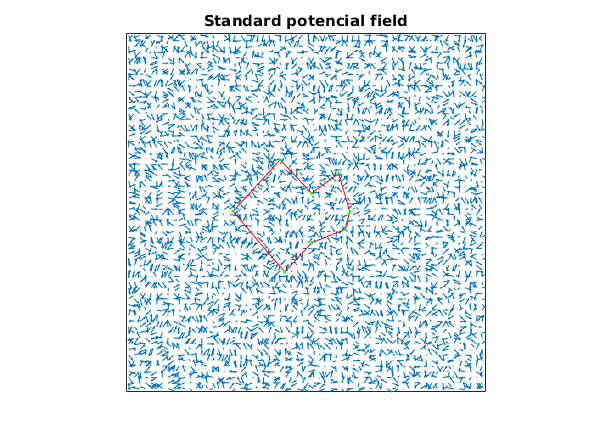
\includegraphics[width=\linewidth]{fig7a.png}
  \caption{The force vector field for the classical snake.}
  \label{fig7a}
\end{subfigure}
\begin{subfigure}{0.49\textwidth}
  \centering
  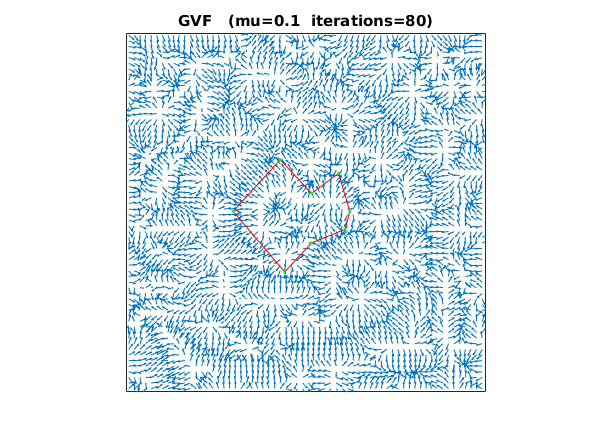
\includegraphics[width=\linewidth]{fig7b.png}
  \caption{The force vector field for GVF ($\mu = 0.1, Iterations=80$).}
  \label{fig7b}
\end{subfigure}
\caption{Force vector fields for heart.pgm.}
\end{figure}

\begin{figure}[H]
\centering
\begin{subfigure}{0.49\textwidth}
  \centering
  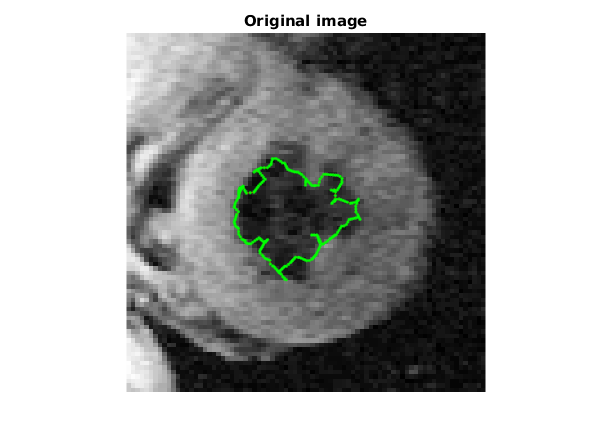
\includegraphics[width=\linewidth]{fig6a.png}
  \caption{The classical snake using initialization heart.mat ($\alpha=0.05, \beta=0, \gamma=1,\kappa=0.6,Dmin=0.5,Dmax=2, Iterations=400$).}
  \label{fig6a}
\end{subfigure}
\begin{subfigure}{0.49\textwidth}
  \centering
  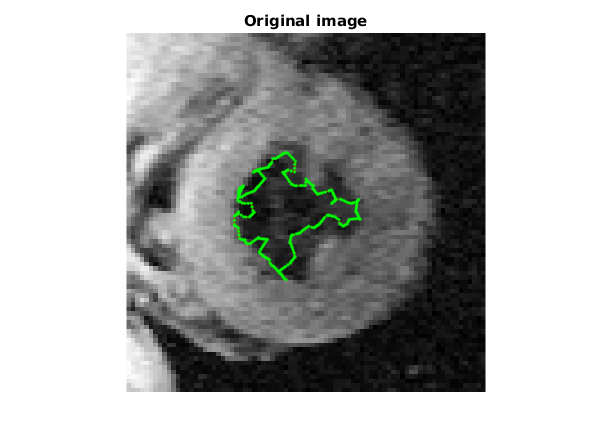
\includegraphics[width=\linewidth]{fig6b.png}
  \caption{The classical snake using initialization heart1.mat ($\alpha=0.05, \beta=0, \gamma=1,\kappa=0.6,Dmin=0.5,Dmax=2, Iterations=400$).}
  \label{fig6b}
\end{subfigure}
\begin{subfigure}{0.49\textwidth}
  \centering
  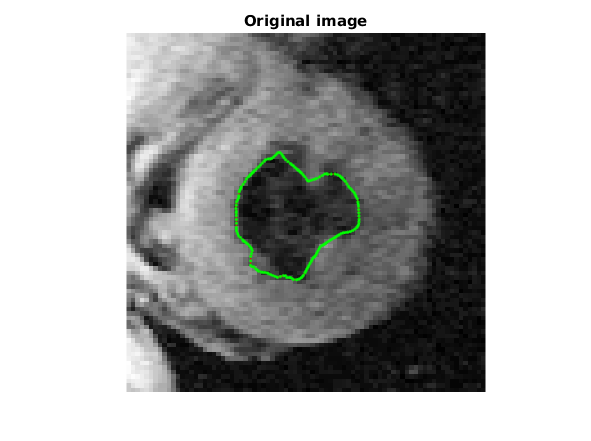
\includegraphics[width=\linewidth]{fig6c.png}
  \caption{The GVF snake using initialization heart.mat ($\mu=0.1, Iterations=90, \alpha=0.05, \beta=0, \gamma=1,\kappa=0.6,Dmin=0.5,Dmax=2, Iterations=400$).}
  \label{fig6c}
\end{subfigure}
\begin{subfigure}{0.49\textwidth}
  \centering
  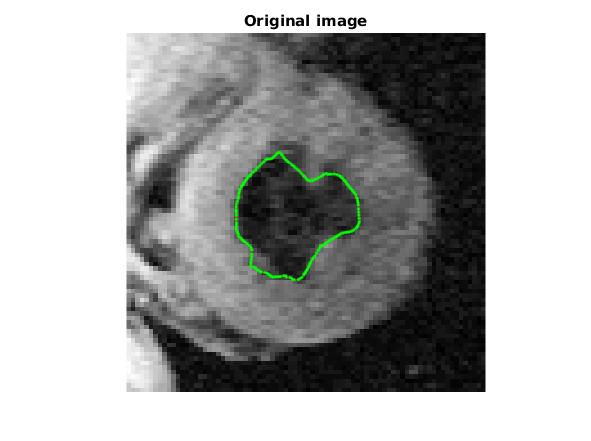
\includegraphics[width=\linewidth]{fig6d.png}
  \caption{The GVF snake using initialization heart1.mat ($\mu=0.1, Iterations=90, \alpha=0.05, \beta=0, \gamma=1,\kappa=0.6,Dmin=0.5,Dmax=2, Iterations=400$).}
  \label{fig6d}
\end{subfigure}
\caption{Results for the non-smoothed heart image.}
\label{fig6}
\end{figure}

\begin{figure}[H]
\centering
\begin{subfigure}{0.49\textwidth}
  \centering
  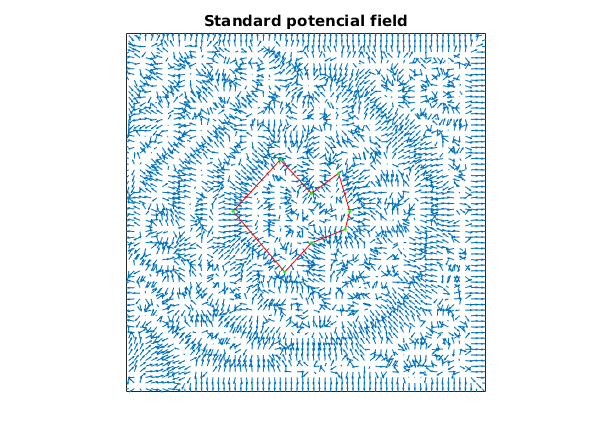
\includegraphics[width=\linewidth]{fig9a.png}
  \caption{The force vector field for the classical snake.}
  \label{fig9a}
\end{subfigure}
\begin{subfigure}{0.49\textwidth}
  \centering
  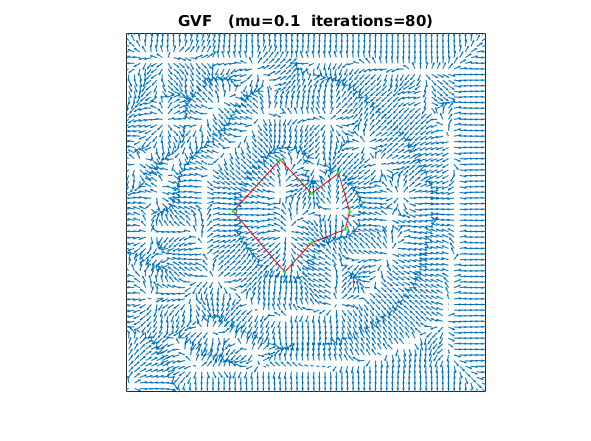
\includegraphics[width=\linewidth]{fig9b.png}
  \caption{The force vector field for GVF ($\mu = 0.1, Iterations=80$).}
  \label{fig9b}
\end{subfigure}
\caption{Force vector fields for the smoothed heart.pgm ($\sigma=3$).}
\label{fig9}
\end{figure}

\begin{figure}[H]
\centering
\begin{subfigure}{0.49\textwidth}
  \centering
  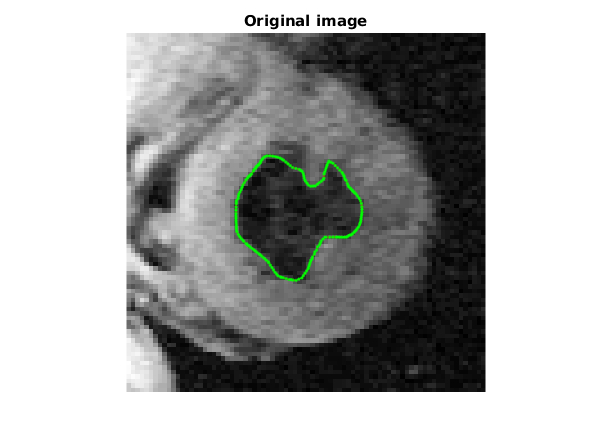
\includegraphics[width=\linewidth]{fig8a.png}
  \caption{The classical snake using initialization heart.mat ($\alpha=0.05, \beta=0, \gamma=1,\kappa=0.6,Dmin=0.5,Dmax=2, Iterations=400$).}
  \label{fig8a}
\end{subfigure}
\begin{subfigure}{0.49\textwidth}
  \centering
  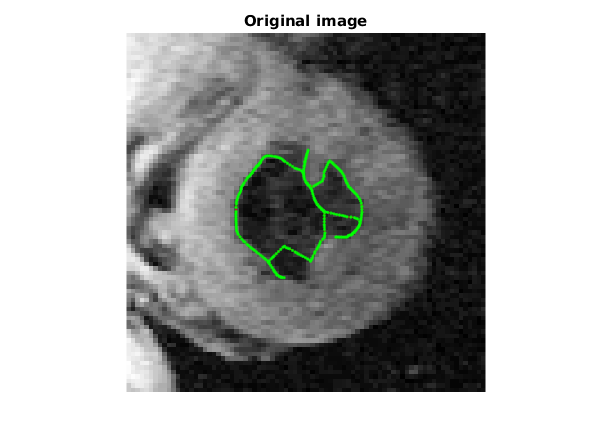
\includegraphics[width=\linewidth]{fig8b.png}
  \caption{The classical snake using initialization heart1.mat ($\alpha=0.05, \beta=0, \gamma=1,\kappa=0.6,Dmin=0.5,Dmax=2, Iterations=400$).}
  \label{fig8b}
\end{subfigure}
\begin{subfigure}{0.49\textwidth}
  \centering
  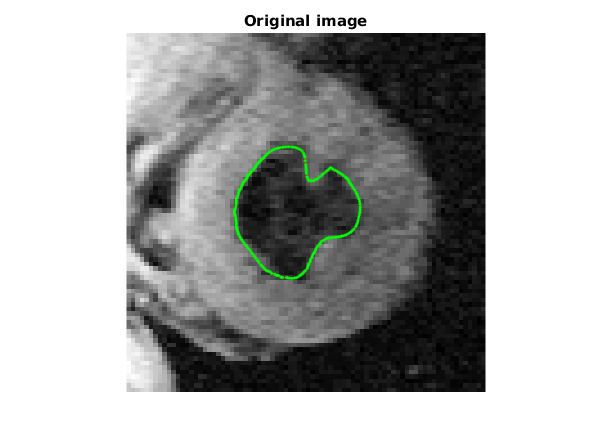
\includegraphics[width=\linewidth]{fig8c.png}
  \caption{The GVF snake using initialization heart.mat ($\mu=0.1, Iterations=90, \alpha=0.05, \beta=0, \gamma=1,\kappa=0.6,Dmin=0.5,Dmax=2, Iterations=400$).}
  \label{fig8c}
\end{subfigure}
\begin{subfigure}{0.49\textwidth}
  \centering
  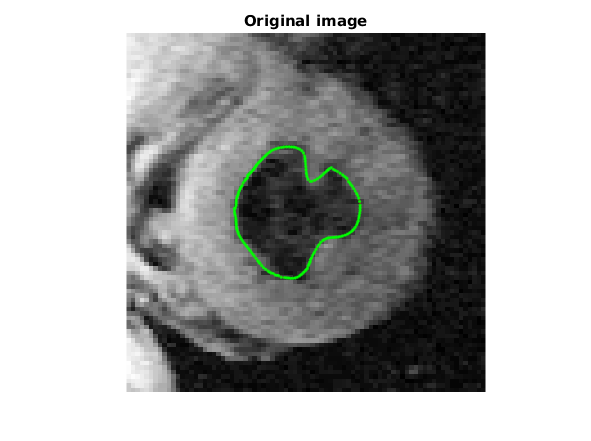
\includegraphics[width=\linewidth]{fig8d.png}
  \caption{The GVF snake using initialization heart1.mat ($\mu=0.1, Iterations=90, \alpha=0.05, \beta=0, \gamma=1,\kappa=0.6,Dmin=0.5,Dmax=2, Iterations=400$).}
  \label{fig8d}
\end{subfigure}
\caption{Results for the smoothed heart image ($\sigma=3$).}
\label{fig8}
\end{figure}

\subsection{}


\end{document}